%\addbibresource{/home/jorgsk/Dropbox/phdproject/bibtex/jorgsk.bib}
\subsection{Model of initial transcription}
Our model is based on a minimal scheme for initial transcription, containing
reactions for i) the NAC, ii) backtracking (here, the
first unscrunching step), iii) unscrunching and abortive RNA release (UAR), and iv)
promoter escape (Figure \ref{fig:model_and_rates}A). The rate constants
for these reactions will be estimated from
fitting to data. In addition, we make use of the assumption that the
probability to backtrack at a template position is equal to the abortive
probability (AP) at that position as calculated by Hsu et. al
\cite{hsu_initial_2006}. In our mode, backtracking is in kinetic competition
with the NAC, which means that the NAC will proceed with probability 100\% -
AP. Thus, for a given rate constant of the NAC, we calculate the rate constant
of backstepping as follows:
\begin{equation}
  b = \frac{\text{NAC}\cdot\text{AP}}{1-\text{AP}}.
  \label{eq:backtrackingcalc}
\end{equation}
Figure~\ref{fig:model_and_rates}B shows the initial transcription kinetic
scheme together with placeholder values for the estimated rate constants.

In this work we use APs obtained both for the absence of GreB (-GreB) and in
the presence of GreB (+GreB). When GreB is present, backtracked complexes may
be rescued by GreB stimulated cleavage of the unaligned 3\ppp end of the
transcript. Therefore, APs obtained in the presence of GreB represent the
probability to both backstep and to avoid rescue by GreB until abortive RNA
release. We assume that GreB-mediated cleavage and subsequent NACs are rapid
steps compared to unscrunching, using the APs obtained in the presence of GreB
as effective backstepping probabilities. All AP values are obtained from Hsu
et al. \cite{hsu_initial_2006}.

\subsection{Implementation and parameter estimation}
The data used for parameter estimation is the distribution of time spent in
abortive cycling \cite{revyakin_abortive_2006}. This data was obtained from
100 individual initial transcription events. For such low copy-number
experiments, there is an inherent stochastic component in the experimental
outcome that derives from the randomness of molecular motion. Indeed, the
rates of transcription elongation obtained by single-molecule experiments show
large standard deviations \cite{adelman_single_2002,
tolic-norrelykke_diversity_2004}. We therefore simulate initial transcription
using stochastic simulations. Specifically, we use the direct method for the
stochastic simulation algorithm \cite{gillespie_exact_1977} as implemented in
the StocPY software \cite{maarleveld_stochpy:_2013}. 

We estimate rate constants by first randomly sample 100000 triplets of the
rate constants for the NAC, promoter escape, and unscrunching and abortive RNA
release. We then use the value for the NAC to calculate rate constants for
backtracking through formula \eqref{eq:backtrackingcalc}. Having thus obtained
all four rate constants, we simulate 100 initial transcription events to find the
predicted distribution of time spent in abortive cycling specific to these
rate constants. This distribution is then compared to the measured values from
Revaykin et.\ al \cite{revyakin_abortive_2006} using the root mean squared
distance metric. The full proceedure is illustrated in Figure
S\ref{fig:parameter_estimation_scheme}.

\begin{figure}
	\begin{center}
        \includegraphics{../illustrations/model_and_rates.pdf}
	\end{center}
    \caption{Kinetic model scheme and reaction rate constants. A) From the
    open complex (OC) transcription proceeds by nucleotide additions cycles
    from one initial transcribing complex (IC) to the next, where each IC is
    identified in subscript by the length of its nascent RNA. Initial
    transcription proceeds until the nascent RNA has reached the
    experimentally obtained maximum size of abortive transcript (MSAT)
    \cite{hsu_initial_2006}. For ICs with an 2nt RNA or longer, there is a
    competition between the nucleotide addition cycle (NAC) and backstepping.
    Backstepping leads to a backtracked state from which further backtracking
    and abortive RNA release occurs, returning RNAP to the open complex. From
    the open complex forward transcription may resume once more. B) Kinetic
    scheme containing placeholder values for the estimated rate constants for
    NAC, $x$, promoter escape, $y$, and unscrunching and abortive release, $z$,
    as well as the rate constants of bakcstepping, $b_i(x)$.}
    \label{fig:model_and_rates}
\end{figure}

